%!TEX program=xelatex

\documentclass[12pt,a4paper,UTF8]{article}
\usepackage[fontset=fandol]{ctex} % Chinese support, using Fandol fonts
\usepackage{graphicx} % Insert images
\usepackage{listings} % Print source code
\usepackage{color} % Color support
\usepackage{booktabs} % Professional table support
\usepackage{pdflscape} % Landscape pages support in PDF
\usepackage{hyperref} % Hypertext links support for cross-referencing
\usepackage{amsmath, amssymb}  % 通常这两个就够了
\usepackage{float}
\usepackage{amsmath} 

\usepackage{ctex} % 支持中文
\usepackage{booktabs} % 支持三线表
\usepackage{array} % 支持列格式定义
\usepackage{geometry}
\geometry{a4paper, margin=2.5cm}




% Customize hyperref format (it's set to no special format here)
\hypersetup{hidelinks}

% Declare directories to search for graphics files for graphicx
\graphicspath{{figures/}{logo/}}

% Define source code style for listings
\lstdefinestyle{cpp-style}{
  language=C++,
  basicstyle=\ttfamily\footnotesize,
  keywordstyle=\bfseries\color[rgb]{0, 0, 1},
  identifierstyle=\color[rgb]{0.5, 0.3, 0.1},
  stringstyle=\color[rgb]{0.6, 0.1, 0.1},
  commentstyle=\itshape\color[rgb]{0.05, 0.5, 0.05},
  backgroundcolor=\color[gray]{0.95},
  numbers=left,
  numbersep=5pt,
  numberstyle=\color[gray]{0.6},
  breaklines=true
}

% Define new command for title page
\newcommand{\reporttitle}[2]{
	\begin{center}
		\LARGE \textsf{#1} \quad #2
	\end{center}
}

\newcommand{\reportinfo}[2]{
  \large\makebox[4em]{\textsf{#1}}\quad\underline{\makebox[18em]{#2}}
}

% The document begins here
\begin{document}
  \begin{titlepage}
    \centering
    \vspace*{\fill}
    
\includegraphics[height=72pt]{NWAFU-logo}\\[48pt] % Change the school logo here (See the logo/ directory) and adjust the height
    {\huge\textsf{机器学习课程大作业}}\\[48pt]
	\reporttitle{}{
		\begin{tabular}{c}
			基于回归学习及流形结构保持的 \\
			无监督特征选择方法实现
		\end{tabular}
	}


\vspace{72pt}


    \reportinfo{课程名称}{机器学习}\\[8pt]
    \reportinfo{专\hspace{\fill}业}{控制工程}\\[10pt]
    \reportinfo{年\hspace{\fill}级}{202X级}\\[10pt]
    \reportinfo{学生姓名}{李雷、韩梅梅}\\[8pt]
    \reportinfo{指导教师}{ABC}\\[8pt]
    \vspace*{\fill}
  \end{titlepage}

  \tableofcontents
  \newpage
	
  \section{引言}
  随着数据挖掘、机器学习和计算机视觉技术的快速发展,研究人员日益面临处理高维数据的挑战。高维数据不仅增加了计算复杂度和存储需求,还可能包含大量冗余和噪声信息,降低算法性能。特征选择作为一种有效的维度降低方法,旨在选择最具代表性的特征子集,已成为高维数据处理的关键技术。特征选择方法通常根据标签信息的可用性分为三类:有监督、半监督和无监督方法。有监督特征选择利用标记数据中包含的判别信息评估特征重要性;半监督方法利用有限的标记数据和大量未标记数据同时进行特征选择;而无监督特征选择则完全不依赖标签信息。考虑到实际应用中高维数据通常缺乏标签,且标注过程成本高昂且耗时,无监督特征选择在实际场景中具有更广泛的应用价值。传统的无监督特征选择方法主要包括过滤方法、包装方法和嵌入方法。过滤方法如方差分析和拉普拉斯得分,通过特征的统计属性选择代表性特征,实现简单但可能忽略特征间的冗余信息;包装方法将特征选择过程与特定学习算法结合,性能较好但计算成本高;嵌入方法将特征选择融入模型构建过程,能够捕获数据多种属性,如局部流形结构和数据相似性。
  
  近年来,基于谱分析的无监督特征选择方法取得了显著进展。这类方法通常包含两个阶段:先构建相似度矩阵学习聚类指示矩阵,再将特征选择嵌入稀疏正则化模型中。其中,多聚类特征选择、无监督判别特征选择、非负判别特征选择和鲁棒无监督特征选择(RUFS)等方法均采用此框架,并在多种任务中表现出良好性能。然而,这些方法通常使用连续伪标签近似真实离散标签,不可避免地引入噪声,影响特征选择效果。另一方面,自表达模型在子空间聚类等领域取得了广泛应用。稀疏子空间聚类和低秩表示等方法利用自表达模型探索样本间相关性,并表现出优于传统聚类算法的性能。自表达模型的扩展版本也被证明能有效处理原始数据中的离群值和噪声。
  
  本文使用一种结合线性回归与流形保持的无监督特征选择方法,其建立了一个基于线性回归的自表达模型,通过特征间的线性重构关系进行特征选择,并引入流形保持约束以保持数据的局部拓扑结构。这种方法避免了传统基于谱分析方法中学习伪聚类标签的步骤,直接从特征间关系出发进行选择,同时通过$\ell_{2,1}$范数正则化实现特征级别的稀疏性。该模型能够同时进行局部结构学习和特征选择,为高维数据分析提供了一种新的无监督特征选择思路。

  \section{相关工作与理论基础}
  \subsection{特征选择方法}
  \subsubsection{有监督特征选择方法}
  有监督特征选择方法利用数据的标签信息评估特征重要性,根据其工作机制可进一步分为三类:过滤式方法、包装式方法和嵌入式方法。
  
  过滤式方法基于统计度量指标评估各特征与目标变量之间的相关性,并选择得分最高的特征子集。典型的过滤式方法包括:信息增益,它计算特征引入后系统熵的减少程度;互信息,度量特征与目标变量的统计依赖性;卡方检验,评估特征与目标类别的独立性;皮尔逊相关系数,衡量特征与连续目标变量的线性相关程度;以及最大相关最小冗余算法,它在选择与目标高度相关特征的同时,最小化所选特征之间的冗余度。过滤式方法计算效率高,独立于后续学习算法,但往往忽略了特征间的交互作用及其对特定学习算法的适应性。
  
  包装式方法将特征选择过程与学习算法性能直接关联,通过特定学习算法在不同特征子集上的表现评估特征重要性。经典的包装式方法包括:向前搜索,从空集开始逐步添加最有贡献的特征;向后消除,从全集开始逐步移除贡献最小的特征;递归特征消除,基于模型权重递归地消除重要性最低的特征;以及遗传算法,通过进化算法搜索最优特征组合。包装式方法能够考虑特征间的相互作用,但计算代价高,且存在过拟合风险,特别是当样本数量有限时。
  
  嵌入式方法将特征选择直接集成到模型训练过程中,在学习算法本身的优化过程中实现特征选择。主要的嵌入式方法包括:L1正则化,通过引入L1范数惩罚项实现稀疏解,自动将不重要特征的权重压缩至零;L1-L2混合正则化,结合L1和L2正则化的优势,既能实现特征选择又能处理特征间的高相关性;决策树特征重要性,基于特征在节点分裂时的信息增益评估重要性;以及基于梯度的特征选择,利用损失函数关于特征的梯度信息评估特征贡献。嵌入式方法平衡了过滤式方法的效率和包装式方法的性能,是实际应用中的常用选择。
  
  \subsubsection{半监督特征选择方法}
  在实际场景中,获取大量标记数据往往成本高昂,而未标记数据则相对容易获取。半监督特征选择旨在同时利用有限的标记数据和大量未标记数据,提高特征选择的效果。标签传播增强的特征选择方法首先利用标记数据和未标记数据构建图模型,通过标签传播算法为未标记数据分配伪标签,然后结合原始标签和伪标签进行特征评估。此类方法包括半监督拉普拉斯得分,它在传统拉普拉斯得分基础上引入标签信息指导特征选择;半监督信息理论特征选择,将互信息准则扩展到半监督环境。共训练框架利用特征空间的多视角性质,在不同视角上交替训练多个分类器,并利用各分类器对未标记数据的预测结果扩充训练集。基于此思想,半监督特征选择可以在不同特征子空间上构建分类器,并通过分类器性能评估特征重要性。
  
 半监督稀疏表示方法将标签信息引入稀疏学习框架,构建同时依赖标记和未标记数据的正则化项。这类方法包括半监督稀疏特征选择,它结合监督学习目标和无监督流形正则化;基于图嵌入的半监督特征选择,通过标签引导的图构建,保留数据的流形结构。虽然半监督特征选择能有效利用未标记数据提高选择性能,但这些方法通常对模型假设敏感,如当数据不满足流形假设或聚类假设时,性能可能显著下降。此外,如何平衡标记数据和未标记数据的贡献也是一个关键挑战。
  \subsubsection{无监督特征选择方法}
  无监督特征选择完全不依赖标签信息,仅基于数据分布特性选择最具代表性的特征。这类方法在标签获取困难或成本过高的场景中具有显著优势,但也面临更大的挑战,因为没有显式的目标信息指导选择过程。基于相似性度量的方法评估特征保留数据内在结构的能力。此类方法包括拉普拉斯得分,它选择能够保持样本局部邻域结构的特征;多集群特征选择,通过谱分析发现能够保持多种聚类结构的特征;以及谱特征选择,它将监督特征选择方法推广到无监督环境,基于图拉普拉斯特征值评估特征重要性。基于稀疏学习的方法利用稀疏正则化实现特征级别的选择。典型方法包括自表达稀疏特征选),通过特征间的稀疏重构关系评估重要性;自适应结构稀疏特征选择,结合局部结构保持和全局稀疏正则化;以及无监督稀疏特征选择,通过构造伪类标签学习特征权重。基于矩阵分解的方法将特征选择问题转化为矩阵分解问题,并通过施加特定约束实现特征选择。此类方法包括主成分分析衍生的特征选择方法,如稀疏主成分分析;非负矩阵分解框架下的特征选择,如嵌入L2,1范数的非负特征选择;以及联合非负矩阵分解特征选择,它同时学习样本表示和特征权重。
  
  深度学习增强的无监督特征选择近年来也受到广泛关注,如基于自编码器的特征选择,通过在重构任务中学习特征重要性;以及基于深度聚类的特征选择,将聚类任务与特征选择联合优化。无监督特征选择虽然适用范围广,但由于缺乏标签信息指导,其表现往往不如有监督方法。如何定义有效的无监督评价指标、如何避免选择到冗余特征、以及如何在特征选择过程中有效融合数据的多种属性,仍是该领域的核心挑战。
  
  \subsection{理论基础}
  \subsubsection{线性回归理论}
  线性回归是统计学和机器学习中最基本也最重要的模型之一,其基本思想是寻找一个线性函数最佳地拟合变量间的关系。在特征选择背景下,线性回归不仅作为一种学习算法,更可视为表达特征间相互关系的框架。
  
  基本线性回归模型假设目标变量可通过输入特征的线性组合来近似:
  $$
  y = \beta_0 + \beta_1 x_1 + \beta_2 x_2 + \cdots + \beta_p x_p + \varepsilon
  $$
  
  
  其中 $y$ 是目标变量,$x_1, x_2, \ldots, x_p$ 是 $p$ 个特征,$\beta_0, \beta_1, \ldots, \beta_p$ 是模型参数,$\varepsilon$ 是误差项。在矩阵形式下,线性回归可表示为:
  
  $$\mathbf{y} = \mathbf{X}\boldsymbol{\beta} + \boldsymbol{\varepsilon}$$
  
  其中 $\mathbf{y} \in \mathbb{R}^{n \times 1}$ 是观测值向量,$\mathbf{X} \in \mathbb{R}^{n \times p}$ 是特征矩阵,$\boldsymbol{\beta} \in \mathbb{R}^{p \times 1}$ 是系数向量,$\boldsymbol{\varepsilon} \in \mathbb{R}^{n \times 1}$ 是误差向量。
  
  最小二乘估计是求解线性回归参数的经典方法,其目标是最小化预测值与观测值之间的平方和误差(Sum of Squared Errors, SSE):
  $$
  \min_{\boldsymbol{\beta}} |\mathbf{y} - \mathbf{X}\boldsymbol{\beta}|_2^2
  $$
  
  
  当 $\mathbf{X}^T\mathbf{X}$ 可逆时,最小二乘解为:
  $$
  \hat{\boldsymbol{\beta}} = (\mathbf{X}^T\mathbf{X})^{-1}\mathbf{X}^T\mathbf{y}
  $$
  
  
  正则化线性回归通过引入惩罚项控制模型复杂度,避免过拟合并实现特征选择。常见的正则化方法包括:
  \begin{enumerate}
  	\item 岭回归):添加L2范数惩罚,控制参数大小: $$\min_{\boldsymbol{\beta}} |\mathbf{y} - \mathbf{X}\boldsymbol{\beta}|_2^2 + \lambda|\boldsymbol{\beta}|_2^2$$
  	\item Lasso回归:添加L1范数惩罚,实现稀疏解和特征选择: $$\min_{\boldsymbol{\beta}} |\mathbf{y} - \mathbf{X}\boldsymbol{\beta}|_2^2 + \lambda|\boldsymbol{\beta}|_1$$
  	\item  弹性网络:结合L1和L2惩罚,平衡两者优势: $$\min_{\boldsymbol{\beta}} |\mathbf{y} - \mathbf{X}\boldsymbol{\beta}|_2^2 + \lambda_1|\boldsymbol{\beta}|_1 + \lambda_2|\boldsymbol{\beta}|_2^2$$
  \end{enumerate}
  
  
  \subsubsection{稀疏学习理论}
  稀疏学习理论为高维数据分析提供了重要理论支撑,其核心思想是利用稀疏性约束从高维噪声数据中提取有意义的模式。在特征选择领域,稀疏性假设认为只有少量特征真正相关且有用,大多数特征可能是冗余或噪声。
  
  稀疏表示假设信号 $\mathbf{x} \in \mathbb{R}^n$ 可以用字典 $\mathbf{D} \in \mathbb{R}^{n \times d}$ 中的少量原子线性组合表示:
  $$
  \mathbf{x} \approx \mathbf{D}\boldsymbol{\alpha}, \quad \text{其中} \quad |\boldsymbol{\alpha}|_0 \ll d
  $$
  
  
  其中 $|\boldsymbol{\alpha}|_0$ 表示向量 $\boldsymbol{\alpha}$ 中非零元素的数量。这一稀疏表示问题可形式化为:
  $$
  \min_{\boldsymbol{\alpha}} |\boldsymbol{\alpha}|_0 \quad \text{s.t.} \quad |\mathbf{x} - \mathbf{D}\boldsymbol{\alpha}|_2 \leq \varepsilon
  $$
  
  
  或等价的拉格朗日形式:
  $$
  \min_{\boldsymbol{\alpha}} |\mathbf{x} - \mathbf{D}\boldsymbol{\alpha}|_2^2 + \lambda|\boldsymbol{\alpha}|_0
  $$
  
  
  不同范数的稀疏正则化在实际应用中,由于 $\ell_0$ "范数"优化是NP难问题,研究者提出了多种凸或非凸近似:
    \begin{enumerate}
  	\item $\ell_1$ 范数(Lasso):$|\boldsymbol{\alpha}|_1 = \sum_i |\alpha_i|$,凸松弛,计算高效
  	\item $\ell_q$ 范数($0 < q < 1$):$|\boldsymbol{\alpha}|_q = (\sum_i |\alpha_i|^q)^{1/q}$,非凸,更接近 $\ell_0$
  	\item  加权 $\ell_1$ 范数:$\sum_i w_i|\alpha_i|$,通过调整权重逼近 $\ell_0$ 范数
  \end{enumerate}
  

  在特征选择背景下,特别重要的是 $\ell_{2,1}$ 范数,定义为矩阵各行 $\ell_2$ 范数之和:
  $$
  |\mathbf{W}|*{2,1} = \sum*{i=1}^{d} \sqrt{\sum_{j=1}^{d} W_{ij}^2} = \sum_{i=1}^{d} |w_i|_2
  $$
  
  
  $\ell_{2,1}$ 范数具有"行稀疏性"(row sparsity)特性,能够将整行系数同时置零,尤其适合特征选择任务。它通过对行内元素应用 $\ell_2$ 范数保持组内结构,同时对行之间应用 $\ell_1$ 范数实现组间稀疏。
  
  \subsubsection{流形学习理论}
  流形学习理论基于一个核心假设:高维数据往往位于低维流形结构上。该理论为处理高维数据提供了重要视角,尤其是在保持数据内在几何结构方面。在特征选择背景下,流形学习理论指导我们选择能够最好地保持数据局部结构的特征子集。
  
  流形假设认为现实世界高维数据(如图像、文本、语音)通常集中在嵌入于高维空间的低维流形上。形式上,假设数据 $\mathbf{X} = {x_1, x_2, \ldots, x_n} \subset \mathbb{R}^d$ 位于维度为 $m$ 的流形 $\mathcal{M}$ 上,其中 $m \ll d$。流形假设的重要性在于:
  
   \begin{enumerate}
  	\item 它解释了高维数据空间的"稀疏性":即数据点不是均匀分布在高维空间中
  	\item 它为降维与特征选择提供了理论基础:关键是保持流形的局部结构
  	\item  它表明数据点之间的真实距离应沿流形测量,而非简单的欧几里得距离
  \end{enumerate}
   
  
  局部线性嵌入是早期的流形学习算法,其核心思想是每个数据点可以通过其近邻的线性组合重构。LLE包括三个步骤:
  
  \begin{enumerate}
  	\item 为每个点 $x_i$ 找到 $k$ 个最近邻 $\mathcal{N}_i$
  	\item 计算重构权重 $W$,最小化重构误差: $$\min_{W} \sum_{i=1}^{n} |x_i - \sum_{j \in \mathcal{N}*i} W*{ij}x_j|^2, \quad \text{s.t.} \quad \sum_{j \in \mathcal{N}*i} W*{ij} = 1$$
  	\item  基于权重 $W$ 计算低维嵌入,保持局部关系
  \end{enumerate}
  
  
  拉普拉斯特征映射利用图论描述数据结构,通过最小化加权距离保持邻近关系。其步骤包括:
  
   \begin{enumerate}
  	\item 构建邻近图,确定点 $x_i$ 和 $x_j$ 是否相连
  	\item 选择权重,通常使用热核(Heat Kernel):$W_{ij} = \exp(-|x_i - x_j|^2/t)$,若点 $i$ 和 $j$ 相连;否则 $W_{ij} = 0$
  	\item  计算低维嵌入 $Y$,最小化: $$\min_{Y} \sum_{i,j} |y_i - y_j|^2_2 W_{ij} = \text{tr}(Y^T L Y)$$ 其中 $L = D - W$ 是图拉普拉斯矩阵,$D$ 是对角矩阵,$D_{ii} = \sum_j W_{ij}$
  \end{enumerate}
  
  
  拉普拉斯矩阵 $L = D - W$ 在流形学习中扮演核心角色,它编码了数据点间的局部关系。拉普拉斯矩阵的重要性质包括:
  
  \begin{enumerate}
  	\item $L$ 是半正定矩阵,特征值非负
  	\item $L$ 的特征向量对应流形上的调和函数
  	\item  二次型 $x^T L x = \frac{1}{2} \sum_{i,j} W_{ij} (x_i - x_j)^2$,测量了加权局部变化
  \end{enumerate}

  
  在特征选择中,拉普拉斯矩阵通常用于构建流形结构保持约束,其形式为:
  $$
  \min_{W} \text{tr}(W^T X^T L X W)
  $$
  
  
  该约束确保特征子集能够保持原始数据的局部流形结构,即如果两个点在原始空间中近似(高 $W_{ij}$ 值),则它们在特征子空间中也应保持近似。
  
  \section{模型建立}
  \subsection{原始问题的抽象化}
  无监督特征选择的核心目标是从原始特征空间中选择最具代表性的特征子集,而不依赖任何标签信息。将问题抽象化,既假设有数据矩阵 $X \in \mathbb{R}^{n \times d}$,其中 $n$ 表示样本数,$d$ 表示特征数。$x_i \in \mathbb{R}^{d \times 1}$ 表示第 $i$ 个样本的特征向量,$f_j \in \mathbb{R}^{n \times 1}$ 表示第 $j$ 个特征在所有样本上的取值。我们的目标是从 $d$ 个特征中选择出 $h$ 个最具代表性的特征($h < d$)。
  
  与传统基于谱分析的无监督特征选择方法不同,本模型不依赖于学习聚类指示矩阵,而是直接分析特征之间的关系。我们基于以下核心思想构建模型:
    \begin{enumerate}
  	\item 自表达性假设:每个特征可以由所有特征的线性组合重构,具有代表性的特征在重构其他特征时应具有较大权重。
  	\item 稀疏性假设:真正重要的特征数量应远少于原始特征总数,因此特征重构权重矩阵应当是行稀疏的。
  	\item  结构保持假设:选择的特征子集应保持数据的原始局部流形结构,确保数据点在重构后的特征空间中保持原有的局部邻近关系。
  \end{enumerate}
 
  
  基于上述思想,我们构建的完整数学模型包含三个关键组成部分:误差项、稀疏性约束和流形结构保持约束。模型的一般形式可表示为:
  
  $$
  \min_{W} \underbrace{\|X - XW\|_F^2}_{\text{误差项}} + \underbrace{\alpha\|W\|_{2,1}}_{\text{稀疏性约束}} + \underbrace{\beta\text{Tr}(W^TX^TL_SXW)}_{\text{流形结构保持约束}}
  $$
  其中,$W \in \mathbb{R}^{d \times d}$ 是特征重构权重矩阵,$\alpha$ 和 $\beta$ 是权重因子,$L_S$ 是基于数据相似度矩阵构建的拉普拉斯矩阵,$\|\cdot\|_F$ 表示F范数,$\|\cdot\|_{2,1}$ 表示$l_{2,1}$范数,$\text{Tr}(\cdot)$ 表示矩阵的迹。本节将详细介绍模型的各个组成部分及其数学推导。
  
  
  \subsection{误差项}
  \subsubsection{基于自表达模型的重构误差}
  我们的特征选择方法以自表达模型为理论基础,该模型最初被广泛应用于子空间聚类领域,并展现出卓越的性能。自表达模型的核心思想是:数据矩阵本身可以作为字典,用于学习数据样本之间的表示关系。我们创新性地将这一思想扩展到特征选择领域,转而关注特征之间的表示关系。设原始数据矩阵为 $X \in \mathbb{R}^{n \times d}$,其中 $n$ 表示样本数量,$d$ 表示特征维度。在自表达模型框架下,每个特征向量可以通过其他特征的线性组合来重构。形式化地,我们有:
  
  $$
  X = XW + E
  $$
  
  
  其中 $W \in \mathbb{R}^{d \times d}$ 是特征重构矩阵(也称为表示矩阵或特征选择矩阵),$E \in \mathbb{R}^{n \times d}$ 是重构误差矩阵。矩阵 $W$ 中的元素 $w_{ji}$ 表示使用第 $j$ 个特征重构第 $i$ 个特征的系数。直观上,如果第 $i$ 个特征对重构其他特征贡献较大,则第 $i$ 行对应的 $w_i$ 的范数会较大,表明该特征
  
  \subsubsection{F 范数与噪声建模}
  在实际应用中,原始数据往往包含各种形式的噪声和扰动,这要求我们的模型具有足够的鲁棒性。为了处理数据中的噪声,我们采用 F范数来度量重构误差,构建如下误差项:
  
  $$
  \|X - XW\|_F^2 = \sum_{i=1}^n\sum_{j=1}^d (X_{ij} - [XW]_{ij})^2
  $$
  F 范数基于均方误差原理,是处理高斯噪声的自然选择。与其他范数相比,F 范数具有以下优势:
   \begin{enumerate}
  	\item F 范数在整个定义域上是可微的,这使得优化过程更加稳定和高效。
  	\item 相比于其他复杂范数,F 范数的计算更为简便。
  	\item  虽然 F 范数对异常值不如某些稀疏范数(如 $\ell_1$ 范数)鲁棒,但它在处理普遍存在的高斯噪声时表现出色。
  \end{enumerate}
  
  
  值得注意的是,虽然实际数据中的噪声分布可能更为复杂,但高斯噪声假设仍然是一个合理且被广泛接受的近似。当然,如果先验知识表明数据中存在特定类型的噪声(如稀疏噪声、脉冲噪声等),可以考虑采用其他相应的范数(如 $\ell_1$ 范数、$\ell_0$ 范数等)来构建误差项。
  
 
 \subsubsection{误差项的矩阵形式}
 为了便于后续优化求解,我们将误差项展开为矩阵形式。首先,根据 F 范数的定义,我们有:
 
 $$
 \|X - XW\|_F^2 = \text{Tr}((X - XW)^T(X - XW))
 $$
 其中 $\text{Tr}(\cdot)$ 表示矩阵的迹。展开上式,得到:
 
 $$
 \|X - XW\|_F^2 = \text{Tr}(X^TX - X^TXW - W^TX^TX + W^TX^TXW)
 $$
 进一步简化,利用矩阵迹的性质 $\text{Tr}(AB) = \text{Tr}(BA)$ 可以得到:
 
 $$
 \|X - XW\|_F^2 = \text{Tr}(X^TX) - 2\text{Tr}(W^TX^TX) + \text{Tr}(W^TX^TXW)
 $$
 在优化过程中,由于 $\text{Tr}(X^TX)$ 是一个与优化变量 $W$ 无关的常数项,可以省略。因此,最终的误差项可以表示为:
 
 $$
 \|X - XW\|_F^2 \propto -2\text{Tr}(W^TX^TX) + \text{Tr}(W^TX^TXW)
 $$
 这种矩阵形式使能够有效地计算目标函数的梯度,从而实现高效的优化求解。
 
 \subsection{稀疏性约束}
 \subsubsection{自表达模型与特征选择}
 我们的方法基于自表达模型这一框架,该框架最初在子空间聚类中被广泛应用,并展现出优异的性能。在特征选择的背景下,自表达模型允许我们探索特征之间的内在关系,并从中识别具有代表性的特征。假设原始数据矩阵为 $X \in \mathbb{R}^{n \times d}$,其中 $n$ 表示样本数量,$d$ 表示特征维度。自表达模型的核心思想是:每个特征向量 $f_i$ 可以通过其他特征的线性组合来重构。形式化地,对于特征向量 $f_i$,我们有:
 
 $$
 f_i = \sum_{j=1}^{d} w_{ji}f_j
 $$
 其中 $w_{ji}$ 表示使用第 $j$ 个特征重构第 $i$ 个特征的系数。集合所有特征的重构系数,我们得到特征选择矩阵 $W \in \mathbb{R}^{d \times d}$。理想情况下,一个具有较强代表性的特征应当在重构其他特征时赋予较大的权重,而不重要的特征则对重构过程贡献较小。
 
 \subsubsection{$\ell_{2,1}$ 范数与行稀疏性}
 为了从 $W$ 中提取具有代表性的特征,我们需要引入稀疏性约束。传统的 $\ell_1$ 范数虽能实现稀疏性,但无法保证矩阵的行稀疏(row sparsity)特性,这对特征选择至关重要。因此,我们采用 $\ell_{2,1}$ 范数作为正则化项,其定义为:
 
 $$
 \|W\|_{2,1} = \sum_{i=1}^{d}\sqrt{\sum_{j=1}^{d}W_{ij}^2} = \sum_{i=1}^{d}\|w_i\|_2
 $$
 其中 $w_i \in \mathbb{R}^{d \times 1}$ 表示矩阵 $W$ 的第 $i$ 行的转置。
 
 $\ell_{2,1}$ 范数的独特之处在于它能够同时实现以下两个关键特性:
    \begin{enumerate}
 	\item 行内致密性:通过对每行应用 $\ell_2$ 范数,保持行内元素的结构完整性;
 	\item 行间稀疏性:通过对行范数之和应用 $\ell_1$ 范数,促使某些行的范数趋近于零。
 \end{enumerate}
 
 这种双重特性使得 $\ell_{2,1}$ 范数成为特征选择任务的理想选择,因为它直接对应了我们的目标:将某些特征(行)的权重完全置零,同时保留其他特征的完整表达能力。
 
  \subsubsection{数值稳定性处理}
 在实际优化过程中,$\ell_{2,1}$ 范数存在一个数值挑战:当某行的 $\ell_2$ 范数趋近于零时,优化问题在该点不可微,这会导致数值计算的不稳定性。为了克服这一问题,我们引入一个平滑化技术,将 $\|w_i\|_2$ 替换为 $\sqrt{w_i^T w_i + \varepsilon}$,其中 $\varepsilon$ 是一个足够小的正常数(通常取 $10^{-16}$)。
 
 这种平滑化技术确保了优化函数在整个参数空间中的可微性,同时当 $\varepsilon$ 趋近于零时,修正后的范数仍然逼近原始的 $\ell_{2,1}$ 范数。因此,我们的稀疏性约束项可以表示为:
 
 $$
 \alpha\sum_{i=1}^{d}\sqrt{w_i^T w_i + \varepsilon}
 $$
 其中 $\alpha > 0$ 是一个权重因子,用于平衡稀疏性约束与其他目标函数项。较大的 $\alpha$ 值会使模型更加注重稀疏性,从而选择更少的特征;而较小的 $\alpha$ 值则允许模型保留更多特征以提高表达能力。
 
 \subsection{流形结构保持约束}
 \subsubsection{局部流形结构表示}
 流形学习理论和谱图理论研究表明,数据的局部流形结构可以通过基于数据点构建的邻近图有效建模。我们采用高斯核函数来计算数据点之间的相似度,构建权重矩阵 $S$。对于任意两个数据点 $x_i$ 和 $x_j$,它们之间的权重可以通过以下公式计算:
 
 $$
 S_{ij} = e^{-\frac{\|x_i - x_j\|^2}{\sigma}}
 $$
 其中 $\sigma$ 是控制高斯核宽度的参数。较大的 $S_{ij}$ 值表示点 $x_i$ 和 $x_j$ 在原始数据空间中非常相似。
 \subsubsection{结构保持约束的抽象表达} \label{332}
 为了保持局部流形结构,我们希望在特征选择后,原始空间中相似的数据点在投影空间中仍然保持相似。具体而言,如果点 $x_i$ 和 $x_j$ 在原始空间中相似($S_{ij}$ 较大),那么它们的重构表示 $W^Tx_i$ 和 $W^Tx_j$ 在特征空间中的距离应该尽可能小。
 
 基于这一原则,流形结构保持约束可以形式化为以下优化问题:
 
 $$
 \min_W \frac{1}{2}\sum_{i,j}\|W^Tx_i - W^Tx_j\|^2_2 S_{ij}
 $$
 注意到当 $S_{ij}$ 较大时,$\|W^Tx_i - W^Tx_j\|^2_2$ 的值会被强制变小,从而保证了原始空间中相近的点在重构空间中仍然相近。
 
 \subsubsection{结构保持约束的拉普拉斯矩阵表示}
 ~\ref{332}~节所描述的优化问题可以进一步简化。利用谱图理论中的拉普拉斯矩阵,我们可以将流形结构保持约束重写为更紧凑的形式。
 
 首先,定义对角矩阵 $D$,其中对角元素 $D_{ii} = \sum_j S_{ij}$ 表示权重矩阵 $S$ 的行(或列)和。然后,拉普拉斯矩阵 $L_S$ 定义为:
 
 $$
 L_S = D - S
 $$
 利用拉普拉斯矩阵的性质,可以得到:
 
 $$
 \frac{1}{2}\sum_{i,j}\|W^Tx_i - W^Tx_j\|^2_2 S_{ij} = \sum_{i=1}^{n}(W^Tx_i)^T(W^Tx_i)D_{ii} - \sum_{i,j=1}^{n}(W^Tx_i)^T(W^Tx_j)S_{ij}
 $$
 进一步简化,得到:
 
 $$
 \frac{1}{2}\sum_{i,j}\|W^Tx_i - W^Tx_j\|^2_2 S_{ij} = \text{Tr}(W^TX^TDXW) - \text{Tr}(W^TX^TSXW) = \text{Tr}(W^TX^TL_SXW)
 $$
 其中 $\text{Tr}(\cdot)$ 表示矩阵的迹,$X \in \mathbb{R}^{n \times d}$ 是原始数据矩阵。
 
 \subsubsection{结构保持约束的最终形式}
 综合上述推导,流形结构保持约束的最终形式为:
 
 $$
 \beta\text{Tr}(W^TX^TL_SXW)
 $$
 其中 $\beta > 0$ 是控制结构保持约束重要性的权重因子。这一约束确保了特征选择过程中数据的局部流形结构得到保持,使得所选特征不仅具有稀疏性,而且能够有效地保持原始数据的几何结构。
 
 \subsection{参数的求解}
 \subsubsection{问题重构}
 回顾目标函数:
 
 $$
 \min_W \|X - XW\|_F^2 + \alpha\|W\|_{2,1} + \frac{\beta}{2}\sum_{i,j}\|W^Tx_i - W^Tx_j\|_2^2 S_{ij}
 $$
 其中,第一项是重构误差项,第二项是L2,1范数正则化项,第三项是结构保持约束项。首先,我们可以将结构保持约束项重写为:
 
 $$
 \frac{1}{2}\sum_{i,j}\|W^Tx_i - W^Tx_j\|_2^2 S_{ij} = \text{Tr}(W^TX^TL_SXW)
 $$
 其中,$L_S = D - S$是拉普拉斯矩阵,$D$是对角矩阵,其对角元素$D_{ii} = \sum_j S_{ij}$。
 
 将$\|W\|_{2,1}$重写为$\sum_i \|w_i\|_2$,其中$w_i$是矩阵$W$的第$i$行,目标函数可以重构为:
 
 $$
 \min_W \|X - XW\|_F^2 + \alpha\sum_i \|w_i\|_2 + \beta\text{Tr}(W^TX^TL_SXW)
 $$
 
 \subsubsection{交替迭代算法}
 由于$\|w_i\|_2$在理论上可能为零,这会导致函数不可微。为避免这种情况,我们将$\|w_i\|_2$重写为$\frac{w_i^Tw_i}{\sqrt{w_i^Tw_i + \varepsilon}}$,其中$\varepsilon$是一个很小的常数。此时,目标函数变为:
 
 $$
 J = \|X - XW\|_F^2 + \alpha\sum_i \frac{w_i^Tw_i}{\sqrt{w_i^Tw_i + \varepsilon}} + \beta\text{Tr}(W^TX^TL_SXW)
 $$
 对$J$关于$W$求导并令其为零,得到:
 
 $$
 \frac{\partial J}{\partial W} = -2(X^TX - X^TXW) + 2\alpha QW + 2\beta X^TL_SXW = 0
 $$
 其中,$Q \in \mathbb{R}^{d \times d}$是对角矩阵,其对角元素为:
 
 $$
 Q_{ii} = \frac{1}{2\sqrt{w_i^Tw_i + \varepsilon}}
 $$
 由于$Q$依赖于$W$,无法直接求解。因此,我们采用交替迭代优化算法:
 
    \begin{enumerate}
 	\item 当$W$固定时,通过以下公式计算$Q$:
 	$$
 	Q_{ii} = \frac{1}{2\sqrt{w_i^Tw_i + \varepsilon}}
 	$$
 	\item 当$Q$固定时,通过求解下列方程得到$W$:
 	$$
 	W = (\beta X^TL_SX + X^TX + \alpha Q)^{-1}X^TX
 	$$
 \end{enumerate}

 
 \subsubsection{模型训练流程}
 完整的交替迭代算法流程如下:
 
 输入:数据矩阵$X \in \mathbb{R}^{n \times d}$,权重矩阵$S$,参数$\alpha$和$\beta$,选择特征的数量$h$。
 
 输出:选择的$h$个特征。
    \begin{enumerate}
 	\item 初始化$Q = I$,$Q \in \mathbb{R}^{d \times d}$
 	\item 计算拉普拉斯矩阵$L_S = D - S$
 	\item  重复以下步骤直到收敛:更新$W = (\beta X^TL_SX + X^TX + \alpha Q)^{-1}X^TX$,随后计算对角矩阵$Q$,其中$Q_{ii} = \frac{1}{2\sqrt{w_i^Tw_i + \varepsilon}}$
 	\item 根据$\|w_i\|_2$的值按降序排列所有特征,选择排名前$h$的特征。
 \end{enumerate}
 
  \subsubsection{收敛性分析}
  
	此模型的收敛性可以通过以下定理证明:
	
	引理1:对于任意正实数$u$和$v$,以下不等式成立:

	$$
		\sqrt{u} - \frac{u}{2\sqrt{v}} \leq \sqrt{v} - \frac{v}{2\sqrt{v}}
	$$
	
	定理1:按照算法中的程序,目标函数单调递减。
	
	证明:假设在第$t$次迭代后得到更新值$\hat{W}$,我们有:
	
	
	$$
		\|X - X\hat{W}\|_F^2 + \alpha\text{Tr}(\hat{W}^TQ\hat{W}) + \beta\text{Tr}(\hat{W}^TX^TL_SX\hat{W}) \leq 
	$$
	
	$$
	\|X - XW\|_F^2 + \alpha\text{Tr}(W^TQW) + \beta\text{Tr}(W^TX^TL_SXW)
	$$

	将$\alpha\sum_i \frac{\varepsilon}{2\sqrt{w_i^Tw_i+\varepsilon}}$加到不等式两边,并代入$Q$的定义,得到:
	
	$$
			\|X - X\hat{W}\|_F^2 + \alpha\sum_i \frac{\hat{w}_i^T\hat{w}_i + \varepsilon}{2\sqrt{w_i^Tw_i+\varepsilon}} + \beta\text{Tr}(\hat{W}^TX^TL_SX\hat{W}) \leq 
	$$
	
	$$
	\|X - XW\|_F^2 + \alpha\sum_i \frac{w_i^Tw_i + \varepsilon}{2\sqrt{w_i^Tw_i+\varepsilon}} + \beta\text{Tr}(W^TX^TL_SXW)
	$$
	基于引理1,有:
	
	$$
	\alpha\sum_i \left(\sqrt{\hat{w}_i^T\hat{w}_i + \varepsilon} - \frac{\hat{w}_i^T\hat{w}_i + \varepsilon}{2\sqrt{w_i^Tw_i+\varepsilon}}\right) \leq
	$$
	
	$$
	 \alpha\sum_i \left(\sqrt{w_i^Tw_i + \varepsilon} - \frac{w_i^Tw_i + \varepsilon}{2\sqrt{w_i^Tw_i+\varepsilon}}\right)
	$$
	将上述两个不等式相加,得到:
	
	$$
	\|X - X\hat{W}\|_F^2 + \alpha\sum_i \sqrt{\hat{w}_i^T\hat{w}_i + \varepsilon} + \beta\text{Tr}(\hat{W}^TX^TL_SX\hat{W}) \leq
	$$
	
	$$
	 \|X - XW\|_F^2 + \alpha\sum_i \sqrt{w_i^Tw_i + \varepsilon} + \beta\text{Tr}(W^TX^TL_SXW)
	$$
	这表明目标函数在迭代过程中单调递减,完成了算法的收敛性的证明。
	
	\subsubsection{计算复杂度分析}
	该算法的主要计算开销来自于矩阵求逆和矩阵乘法操作。每次迭代中,更新$W$的计算复杂度为$O(d^3 + nd^2)$,其中$d$是特征数量,$n$是样本数量。更新对角矩阵$Q$的计算复杂度为$O(d)$。
 
 \section{实验设计}
 \subsection{数据集来源}
 本文使用课程实验环节中所使用的MNIST手写体数字数据集进行实验设计和结果展示,以探究正则化参数($\alpha$)和流形保持权重参数($\beta$)对模型性能的影响。MNIST数据集是一个广泛用于训练各种图像处理系统的大型手写数字数据库,也被广泛用于机器学习领域的训练和测试。这个数据库是图像识别数据集中最受欢迎的之一。这些样本都是由美国的高中生和美国人口调查局的员工手写的。每个图像都是28x28像素的灰度图像,代表了0到9的数字。这个数据集已经被广泛用于机器学习和深度学习的研究,包括图像分类、数字识别等任务。
 
 \subsection{实验环境}
 本研究所使用的计算机处理器为AMD R5-5600X,GPU为NVIDIA RTX 4060(16GB),内存为32.0 GB,操作系统为Ubuntu 20.04 LTS。采用Python(3.9.12)作为编程语言,Origin 2022用于数据可视化。
 
 \subsection{评价指标}
 \subsubsection{分类准确率(Acc)}
 聚类准确率是评估聚类质量的一种直观度量,它反映了聚类结果与真实类别标签的匹配程度。然而,由于聚类算法产生的簇标签与真实类别标签之间不存在天然的一一对应关系,本文首先找到最优的标签映射,然后计算匹配率。
 
 聚类准确率的计算步骤如下:
    \begin{enumerate}
 	\item 构建代价矩阵:首先构建一个代价矩阵 $G \in \mathbb{R}^{n_1 \times n_2}$,其中 $n_1$ 是真实类别数量,$n_2$ 是预测聚类数量。矩阵元素 $G_{ij}$ 表示同时属于真实类别 $i$ 和聚类簇 $j$ 的样本数量。
 	\item 寻找最优映射:使用匈牙利算法求解最优匹配问题,找到真实标签和聚类标签之间的最佳一一对应关系,使得匹配样本总数最大化。
 	\item  计算准确率:基于最优映射,计算正确分类的样本比例: 
 \end{enumerate}



 $$
 ACC = \frac{\sum_{i=1}^{n} \delta(y_i, map(c_i))}{n}
 $$
 
 
 其中,$y_i$ 是第 $i$ 个样本的真实标签,$c_i$ 是其聚类标签,$map(\cdot)$ 是由匈牙利算法确定的最优映射函数,$\delta(x,y)$ 是指示函数,当 $x=y$ 时取值为1,否则为0,$n$ 是样本总数。
 \subsubsection{归一化互信息(NMI)}
  标准化互信息是基于信息论的聚类评价指标,它衡量了两个标签分布之间的相互依赖性,不受标签具体值的影响。NMI计算真实标签分布与预测聚类分布之间共享的信息量,并通过归一化处理使其值域限定在[0,1]区间内。
 
 NMI的计算公式为:
 $$
 NMI(Y, C) = \frac{I(Y; C)}{\sqrt{H(Y) H(C)}}
 $$
 其中:
 \begin{itemize}
 	\item $I(Y; C)$ 是真实标签 $Y$ 和聚类结果 $C$ 之间的互信息
 	\item $H(Y)$ 和 $H(C)$ 分别是 $Y$ 和 $C$ 的熵
 	\item 互信息 $I(Y; C) = \sum_{y \in Y} \sum_{c \in C} p(y, c) \log \frac{p(y, c)}{p(y)p(c)}$
 	\item 互信息 $I(Y; C) = \sum_{y \in Y} \sum_{c \in C} p(y, c) \log \frac{p(y, c)}{p(y)p(c)}$
 \end{itemize}
 
 
 \newpage
 
 \section{实验结果分析}

  \begin{figure}[H]
	\centering
	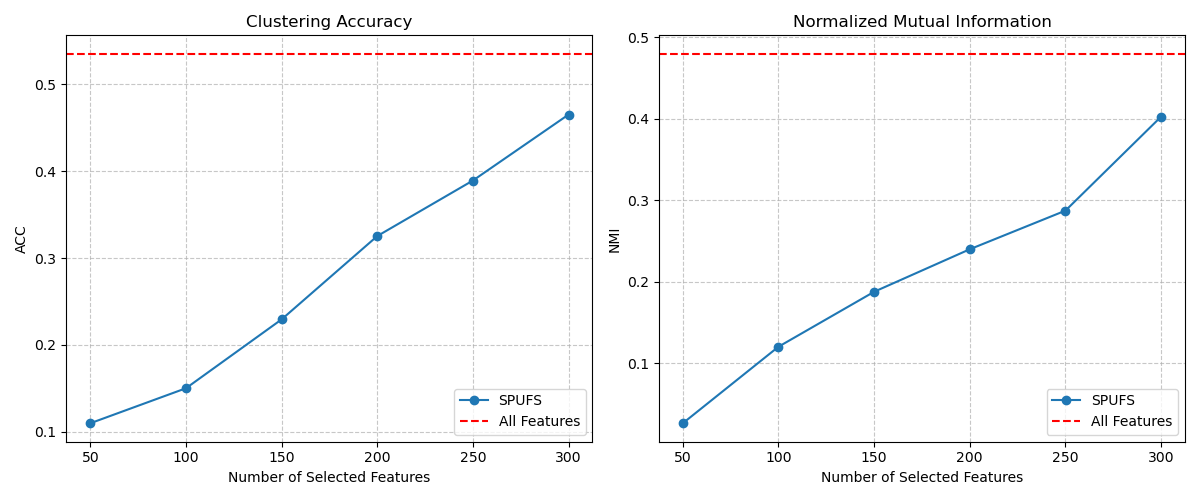
\includegraphics[width=1.0\textwidth]{./results/feature_selection_results}
	\caption{特征选择性能曲线}
	\label{特征选择性能曲线图}
\end{figure}
 
 图 \ref{特征选择性能曲线图} 展示了在固定参数($\alpha$=1.0 和 $\beta$=1.0)不同特征数量下的聚类性能变化。图中左半部分展示了Acc随所选特征数量增加的变化趋势,从50个特征时的约0.11单调增加至300个特征时的约0.47,右半部分展示了归一化互信息 NMI 的类似趋势。两个性能指标均随特征数量的增加而提升,且增长率在特征数量较少时更为显著,随着特征数量接近300,增长速率逐渐放缓,表现出典型的边际效益递减特性。图中水平红色虚线代表使用全部特征的基准性能,算法在仅选择300个特征(相比原始特征空间的大幅降维)的情况下,已能达到接近全特征性能的水平。这一结果有力证明了该算法在识别高信息量特征子集方面的有效性,同时也说明了在保持聚类性能的前提下,可以通过结构保持无监督特征选择算法实现显著的维度降低。曲线的单调上升特性进一步表明,算法能够根据特征重要性有效排序,为不同维度约束条件下的特征选择提供了灵活选择。
 

 
  \begin{figure}[H]
 	\centering
 	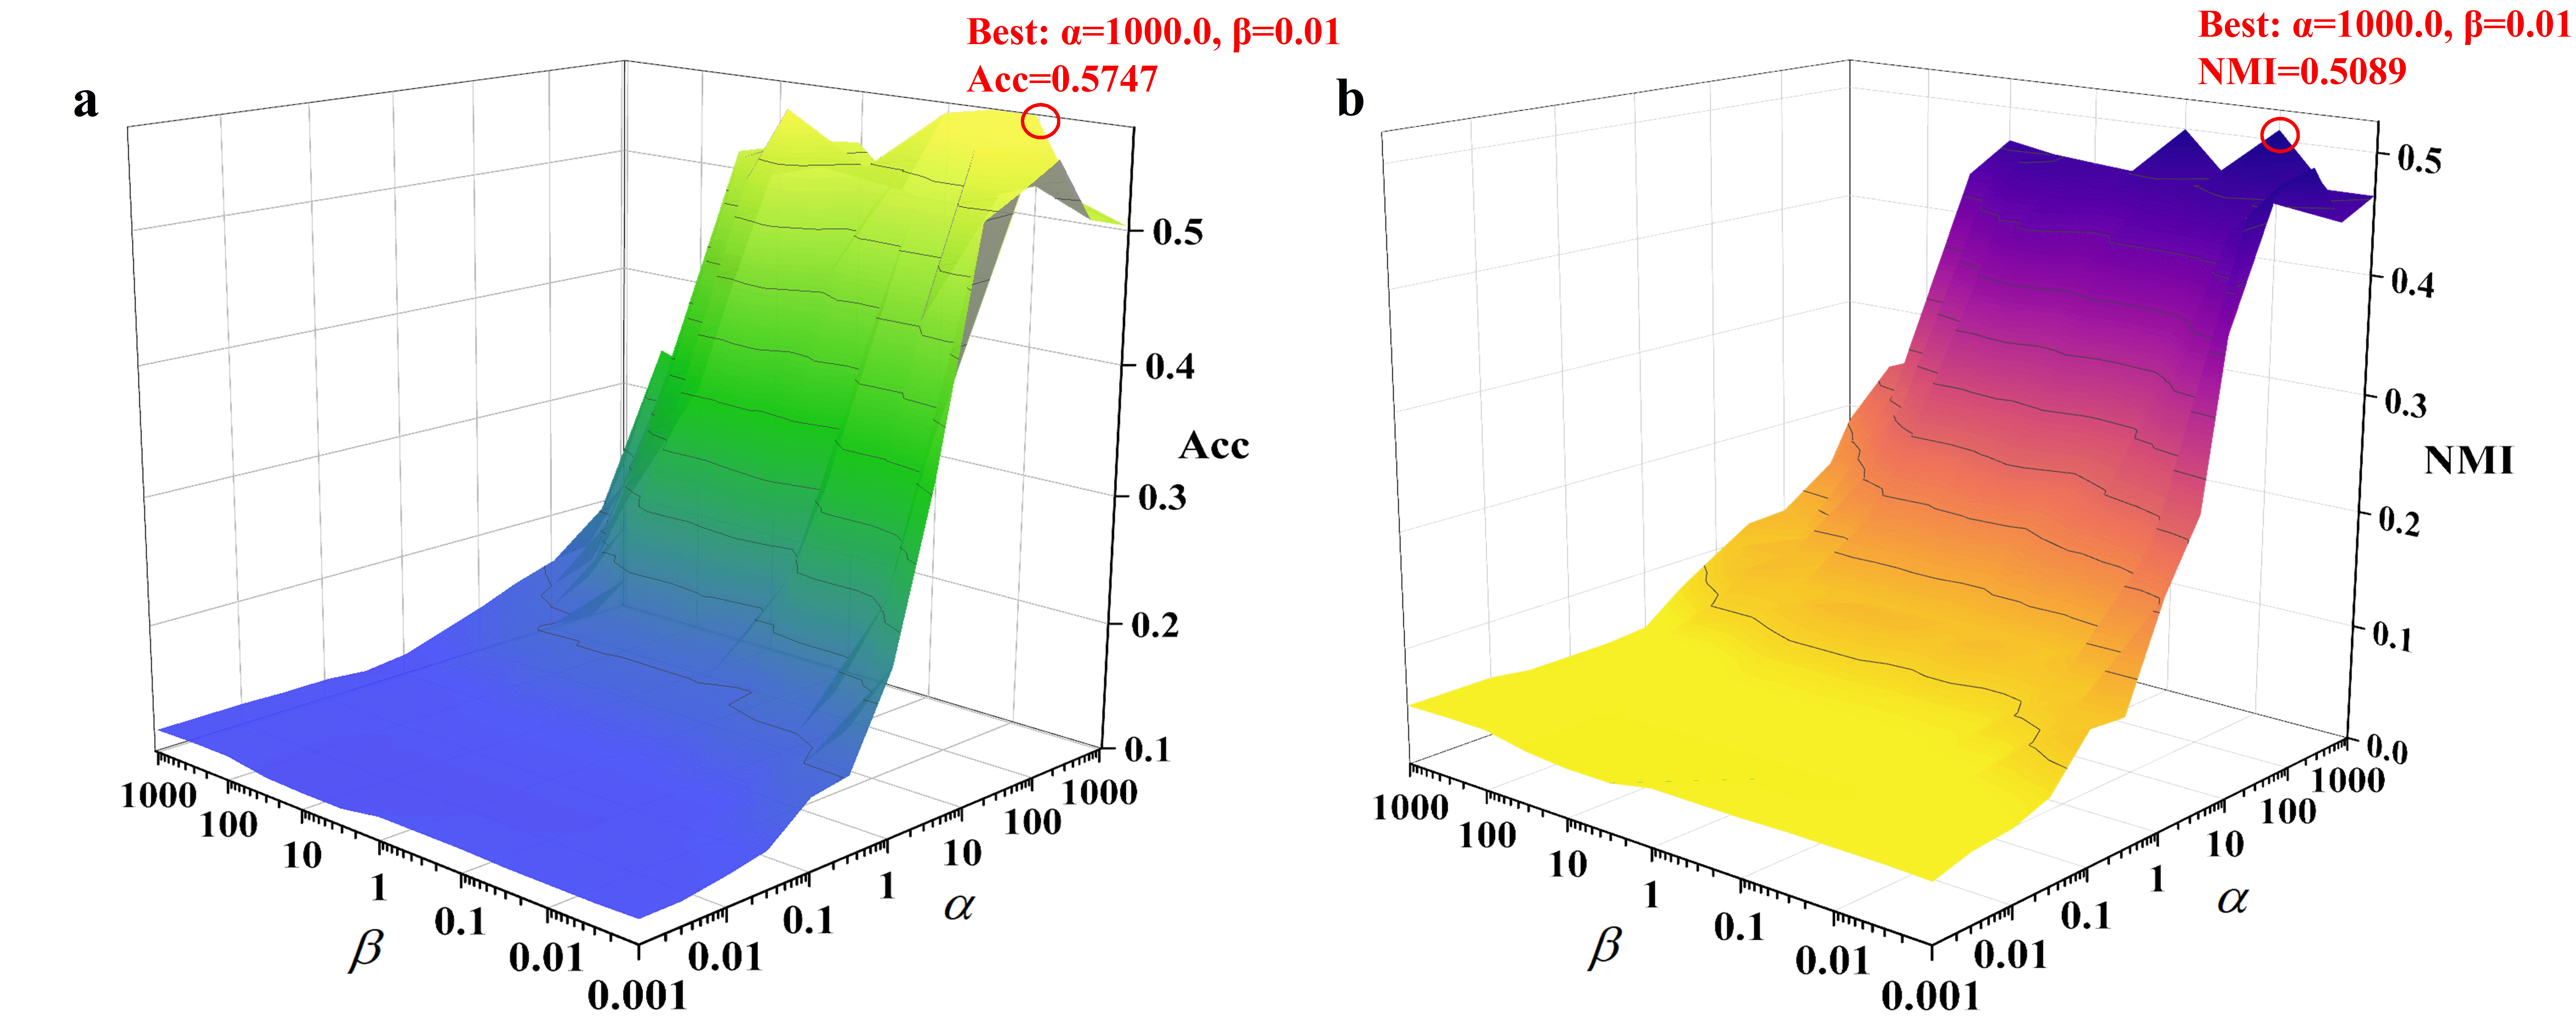
\includegraphics[width=1.0\textwidth]{./results/compare}
 	\caption{Acc(a)和NMI(b)的超参数网格搜索结果}
 	\label{超参数网格搜索结果}
 \end{figure}
 图 \ref{超参数网格搜索结果} 展示了结构保持无监督特征选择算法的参数敏感性分析三维曲面图展示了超参数$\alpha$和$\beta$对聚类性能的复杂影响。图中清晰呈现的性能表面表明,随着正则化参数$\alpha$的增加,Acc和NMI均呈现显著上升趋势,特别是当$\alpha$值达到较高水平时。同时,结构保持参数β表现出明显的非单调影响,其最优值位于较小区域($\beta$=0.01),此时算法达到最佳性能(Acc=0.5747,NMI=0.5089)。这一现象表明,虽然适当的结构保持约束有助于保留数据内在几何特性,但过强的约束可能会对特征选择产生不利影响。图中性能曲面在参数空间中的陡峭变化进一步揭示了该算法对参数选择的高敏感性,强调了在实际应用中精确参数调优的重要性。特别值得注意的是,在高$\alpha$值和低$\beta$值区域形成的"高原"区域,表明在特定参数范围内算法能够保持相对稳定的高性能,为实际应用提供了可靠的参数选择指导。
 
   \begin{figure}[H]
 	\centering
 	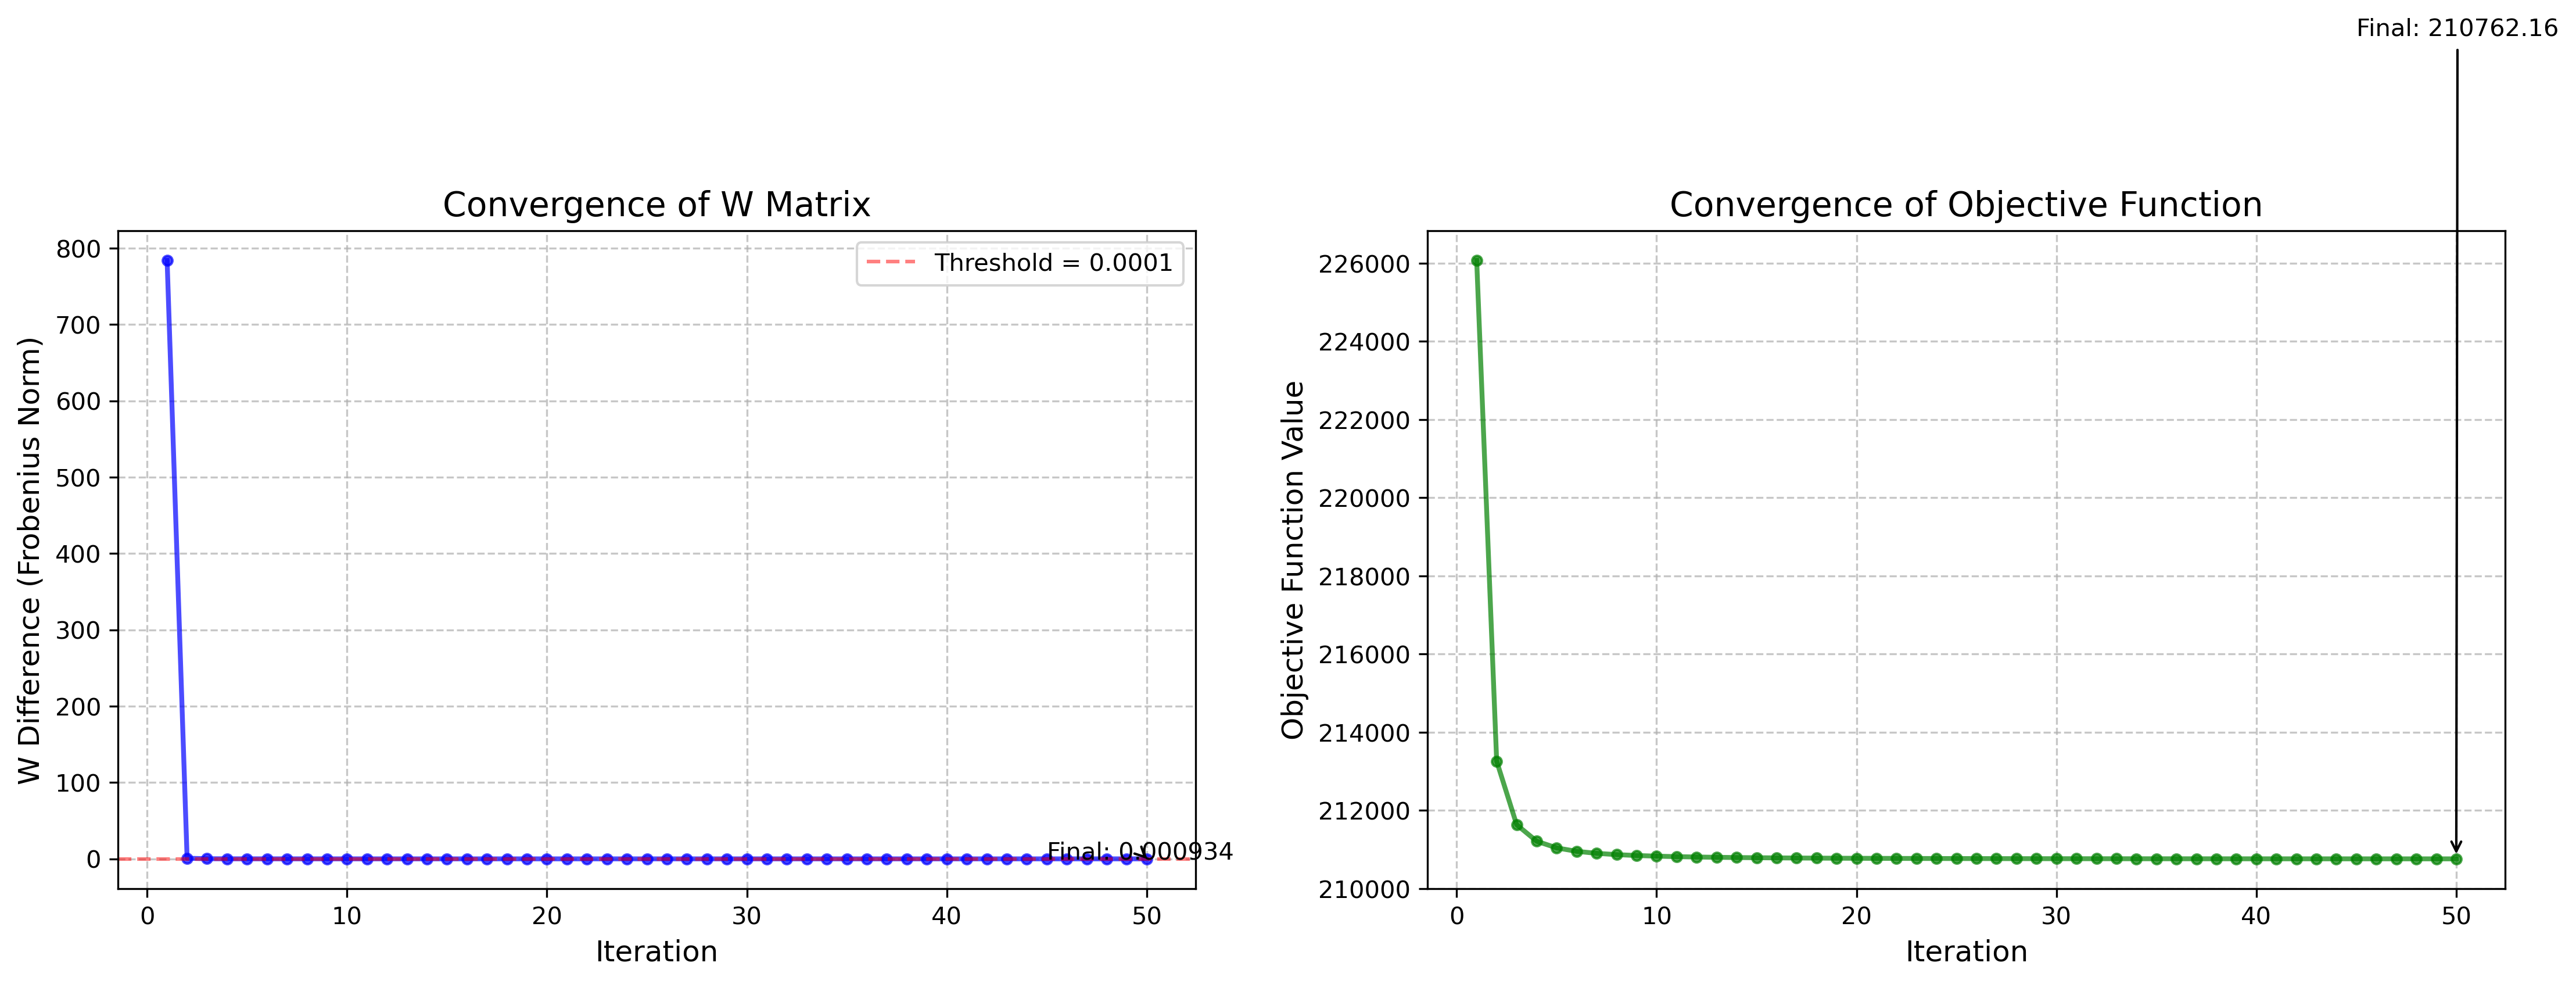
\includegraphics[width=1.0\textwidth]{./results/convergence_best_params_a1000.0_b0.01}
 	\caption{收敛性曲线}
 	\label{收敛性曲线图}
 \end{figure}
 
 如图 \ref{收敛性曲线图} 所示为结构保持无监督特征选择算法的收敛性分析图,W矩阵差异图展示了算法在迭代过程中的快速收敛特性,F范数差值从初始的约800在极少数迭代内(约2-3次)便急剧下降至接近零,随后保持在极低水平,最终达到0.000934,远低于设定的收敛阈值0.0001(红色虚线所示)。而目标函数值收敛图同样呈现出良好的下降特性,从初始值约226,000快速降至约211,000,并在后续迭代中继续缓慢优化至210,762.16。两图均展现出典型的凸优化问题收敛模式,初期快速下降后逐渐趋于平稳。这种收敛模式证实了基于回归学习及流形结构保持的无监督特征选择方法所采用的交替优化策略的高效性,以及其在处理大规模特征选择问题时的计算稳定性。特别是W矩阵差异的快速收敛表明,算法能够在较少迭代次数内找到稳定的特征权重表示,这对于处理大规模高维数据的实际应用具有重要意义。
 
 
 \section{结论}
 本文使用了一种结合线性回归与流形保持的无监督特征选择方法,通过建立基于线性回归的自表达模型并引入流形保持约束,在MNIST数据集上展现出显著性能。实验结果表明,该方法能在仅选择少量特征的情况下达到接近全特征的聚类性能,且参数敏感性分析揭示了正则化参数$\alpha$与流形保持参数$\beta$的复杂影响关系,其中最佳性能出现在较高$\alpha$值和较低$\beta$值区域。方法的显著优势在于避免了传统伪标签学习步骤,直接从特征间关系出发进行选择,同时通过$\ell_{2,1} $范数实现特征级稀疏性,其快速收敛的交替迭代算法也使其适用于大规模高维数据处理。虽然算法对参数选择较为敏感,但在合适参数配置下能够有效平衡特征稀疏性与数据结构保持,未来工作将探索自适应参数设置、降低计算复杂度以及扩展到其他领域的高维数据分析中。
 
 
	\section{小组成员分工情况}
	
	本小组成员分工情况如表 \ref{小组成员及其分工情况} 所示。
	\begin{table}[htbp]
		\centering
		\caption{小组成员及其分工情况}
		\renewcommand{\arraystretch}{1.4} % 增加行距
		\begin{tabular}{
				>{\centering\arraybackslash}p{3cm} 
				>{\centering\arraybackslash}p{4cm} 
				>{\centering\arraybackslash}p{7cm}
			}
			\toprule
			\textbf{学号} & \textbf{小组成员姓名} & \textbf{负责部分} \\
			\midrule
			2024111111 & 李雷 & 环境搭建、编写并运行模型代码 \\
			2024222222 & 韩梅梅   & 搜索相关文献、辅助编写代码 \\
			\bottomrule
		\end{tabular}
		\label{小组成员及其分工情况}
	\end{table}


\begin{thebibliography}{99}  % 参数是最大编号宽度,99 可容纳两位数编号
	\bibitem{ref1}
	Lu Q, Li X, Dong Y. Structure preserving unsupervised feature selection[J]. Neurocomputing, 2018, 301: 36-45.

\end{thebibliography}

\end{document}